\section{Evaluation}\label{sec:evaluation}

In this section, we compare \gsnfs{} against the state of the art, using two popular \dgs{} data sets.

\subsection{Methodology}\label{sec:methodology}

%% \begin{outline}
%%   Describe:
%%   \begin{itemize}
%%   \item Implementation
%%   \item Experimental machine details: Precision/Jetson
%%   \item Baselines + datasets
%%     \begin{itemize}
%%     \item V3~\cite{v3}: person + HiFi4G (7 videos)
%%     \item QUEEN~\cite{queen}: scene + N3DV (6 videos)
%%     \item For each, post-training schemes: LTS-Draco, Ours, MesonGS, V3-2D, GPCC
%%     \end{itemize}
%%   \item Metrics
%%     \begin{itemize}
%%     \item Objective quality: PSNR/SSIM/LPIPS
%%     \item Encode and decode latency (decode on Jetson/Precision or both)
%%     \item Compression ratio
%%     \end{itemize}
%%   \item Experiment:
%%     \begin{itemize}
%%     \item All frames, all videos and tabulate results
%%     \end{itemize}
%%   \end{itemize}
%% \end{outline}

\parab{Implementation.}
%
We have implemented \gsnfs{} in Python.
%
It uses custom CUDA kernels for the octree encoder/decoder (\cref{sec:gpu-octree}), RAHT (\cref{sec:gpu-raht}), and RLGR  (\cref{sec:quant-entr-coding}).
%
It compresses position using the ANS entropy coder from NVIDIA's nvCOMP library~\cite{nvidia_nvcomp} and implements KLT decorrelation and quantization in PyTorch~\cite{pytorch}; these run on the GPU.
%
Most of the data and intermediate tensors use PyTorch.
%
%% We use \texttt{float32} precision (\gsnfs also supports \texttt{float64, float16}) for RAHT, while we use \texttt{uint32} for quantization and RLGR.
%% %T
%% The morton codes use \texttt{uint64} to support octree depth up to 21.
%
%The entire encode and decode pipeline is GPU-resident: \gsnfs{} reads each frame from disk into GPU memory, processes it through all encoder stages of \gsnfs{} entirely in GPU, then copies the final compressed bitstream to the host.
%
%The decoding process is similar but in reverse.

\parab{Hardware.}
%
Most experiments run on a PC equipped with an NVIDIA RTX 4500 Ada Generation GPU (24~GB VRAM), 128~GB system RAM, and Intel(R) Xeon(R) w7-2475X with 20 physical cores (40 threads with hyperthreading).
%
Mobile decoding runs on an NVIDIA Jetson.

\parab{Baselines.}
%
We compare \gsnfs{} against four post-training compression baselines:
\begin{description}
  \item[\vthree{}-2D~\cite{v3volumetric}]
  %
  maps Gaussian attributes to 2-D image stacks, one per attribute channel, and compresses the resulting images with a H.264 codec using \texttt{x264} from FFmpeg~\cite{ffmpeg}.
  %
  It compresses each channel of attributes into a single MP4 stream, where frames for that attribute form a group of pictures (GOP), and a single quantization parameter (QP) controls the quality-size tradeoff.
  %
  It splits the position of Gaussians into MSB and LSB, where QP for MSB is 0 (lossless) and QP for LSB is the QP passed to the encoder (default: 25).
  %
  \vthree{}-2D caps QPs for rotation and scale attributes to 22, and quantizes all other attributes (position LSB, color, opacity) with the same QP (default: 25).
  %
  It compresses each attribute channel using one call of the H.264 encoder, resulting in 62 MP4 files per GOP (default: 20).

  \item[MesonGS~\cite{mesongs}] is a partly GPU-accelerated codec that uses an octree for geometry, RAHT and block quantization for attributes, vector quantization for higher-degree SH coefficients, and LZ77 for entropy coding. 
  %
  We use the authors' default parameters.

  \item[G-PCC~\cite{gpcc}] Wang \textit{et al.}~\cite{gpcc-adaptive} use G-PCC to compress static \gs, and adapt octree depth for voxelization to preserve quality.
  %
  This requires fine-tuning of Gaussians after voxelization to reach high quality.
  %
  To obtain a baseline that directly extends G-PCC to \dgs{} videos, we implement a simplified version of \cite{gpcc-adaptive} (without adaptive voxelization and fine-tuning).
  %
  The approach uses RAHT for color and opacity (lossy, depending on QP) and hierarchical neighborhood prediction for rotation and scale (lossless).

  \item[LTS-Draco~\cite{LTS,mga}] 
  %
  uses modified Draco to independently compress each \gs{} frame on the CPU. 
  %
  The number of quantization bits per attribute is configurable (default: 16 bits for all attributes, compression level 10).
\end{description}
%
In each case, we use the implementations provided by the authors.
%
Moreover, these baselines use qualitatively different compression techniques for \dgs{}: 2D codecs~\cite{v3volumetric}, Draco~\cite{LTS}, and G-PCC~\cite{mesongs,gpcc-adaptive}.

\parab{Datasets.}
%
We evaluate on two widely-used \dgs{} video datasets spanning diverse content types:
\begin{description}
  \item[HiFi4G~(7 sequences)] contains person-centric captures of actors performing various actions, with $200$ frames per sequence. We use \gs{} models trained using \vthree~\cite{v3volumetric} with SH coefficient degrees $0..3$ (${\sim}120$K--$300$K Gaussians per frame).

  \item[Neural 3D Video (N3DV)~(6 sequences)] contains full-scene captures of indoor table-top activities with day and night lighting, each with~300 frames. We use models trained with QUEEN~\cite{queen} (without its in-training compression) with SH degrees $0..2$ (${\sim}150$K--$400$K Gaussians per frame).
\end{description}

\parab{Metrics.}
For each approach, we report measures of:
%
(1) \textit{visual quality} based on PSNR computed on rendered test views of the decompressed frames against the uncompressed ground truth (we use the test views used by \vthree and QUEEN);
%
(2) \textit{per-frame encode} and \textit{decode latency} in milliseconds (ms); and
%
(3) \textit{compression efficiency} in terms of \gs{} frame size after compression.
%
We describe the precise metrics below.

%
%% We also log CPU utilization, GPU utilization, and memory consumption during each pipeline's execution via \texttt{psutil} and \texttt{pynvml}.
%% \raj{Might remove CPU and GPU util}

\subsection{Baseline Comparison}\label{sec:baseline-comparisons}

%% \begin{outline}
%%  o 
%% This section focuses only on compression, since other approaches are not bandwidth-adaptive. We study bandwidth-adaptivity in the next section.

%% Approach: pick the best quality QP value for all other competing approaches, and for us, the knee of the curve. Explain why we do it this way.

%%   Discuss in order: (these can be under different paragraph headings)
%%   \begin{itemize}
%%   \item Quality
%%   \item Latency
%%o   \item Compression ratio
%%   \end{itemize}

%%   As part of discussing the results, think of additional graphs or figures that you think are needed to explain some of the results.
  
%% \end{outline}

\parab{Methodology.}
%
This section compares \gsnfs{} against all baselines at a single operating point.
%
For competing approaches, we select the default parameters for compression, such as QP, octree depth, bit-depth, \etc, that we either found in the corresponding paper or source code.
%
For \gsnfs{}, we use parameters that give us the same quality (PSNR) on the first frame of a sequence as the default setting for each approach.
%
For instance, if, on the first frame of sequence $S$, \vthree{}-2D has a PSNR of $p$, we find a parameter setting for \gsnfs{} (using the technique described in \cref{sec:rd-curves}) whose PSNR for the first frame on $S$ is close to $p$.
%
This results in a pair-wise comparison between \gsnfs{} and each baseline.

% \ao{Why every 10th frame? This makes sense for methods that do not use motion prediction (e.g., ours) but if you encode the attributes of every 10th frame with a video encoder (which uses motion estimation and compensation) you are putting it at a disadvantage as the motion prediction is best when it applies to consecutive frames.}
We use these settings to encode, decode, and estimate PSNR and compression sizes for every 10th frame\footnote{For \vthree{}-2D, we compute the size of a frame as the average size of the GOP that it belongs to.} of every sequence in the two datasets listed above.
%
We do this primarily because some of the baselines~\cite{mesongs,gpcc-adaptive} have exceedingly high encode/decode latencies, rendering an exhaustive evaluation intractable.
%
Then, we compute, for each sequence: (a) the average per-frame encode latency, (b) the average per-frame decode latency, (c) the average per-frame PSNR difference between \gsnfs{} and the baseline (the \dpsnr{}), (d) average per-frame size ratio between \gsnfs{} and the baseline (the \textit{relative compression ratio}, or \rcr{}).

\begin{table}[t]
  \centering
  % \footnotesize
  \begin{tabular}{l|rr|rr}
    \hline
    & \multicolumn{2}{c|}{\textbf{N3DV (QUEEN)}} & \multicolumn{2}{c}{\textbf{HiFi4G (\vthree)}} \\
    \textbf{Pipeline} & Enc.\ (ms) & Dec.\ (ms) & Enc.\ (ms) & Dec.\ (ms) \\
    \hline\hline
    \textbf{\gsnfs{}} & \textbf{23} & \textbf{21} & \textbf{18} & \textbf{14} \\
    \vthree{}-2D & 370 & 290 & 1098 & 341 \\
    LTS-Draco   & 400 & 158 & 156 & 91 \\
    G-PCC        & 8804 & 6928 & 6101 & 3650 \\
    MesonGS     & 28996 & 1096 & 144953 & 535 \\
    \hline
  \end{tabular}
  \caption{Per-frame encode and decode latency (ms).}
  \label{tab:baseline-latency}
\end{table}

\subsubsection{Encode-Decode Latency}\label{sec:latency}

\cref{tab:baseline-latency} summarizes per-frame encode and decode times aggregated across all sequences within each dataset.
%
We do this because, within a dataset (\textit{e.g.}, HiFi4G), there is little variability in encode and decode times across sequences, since all sequences are person-centric.
%
\cref{app:coding-latency} contains a more detailed breakdown.

% \ao{below sections do not need to repeat the data that is already in the table (e.g., 23ms, 18ms, etc.) This can be left in the table and the text can focus on a qualitative discussion or give the 9-17X decoding speed results.}
\gsnfs{} achieves ${\sim}23$~ms encode and ${\sim}21$~ms decode on N3DV, and ${\sim}18$~ms encode and ${\sim}14$~ms decode on HiFi4G---well under the 33~ms budget for 30 frames-per-second (fps).

LTS-Draco, the next fastest baseline, is \textbf{9--17$\boldsymbol\times$ slower than \gsnfs{} for encoding} and \textbf{7--8$\boldsymbol\times$ slower for decoding}.
%
Draco encoding and decoding could potentially be made faster using coarse-grained CPU parallelism~\cite{meshreduce,vivo,metastream}, but this trades off compressibility.

Though 2D video codecs are fast, \vthree{}-2D's several hundred milliseconds to encode decode, due to the overhead of calling video encoder sequentially for each channel\footnote{\vthree{}-2D encodes and decode the full scene N3DV dataset faster than the HiFi4G person-centric dataset, because, on the former dataset, QUEEN does not produce degree-3 SHs.};
It is \textbf{16--61$\boldsymbol\times$ slower than \gsnfs{} for encoding} and \textbf{14--24$\boldsymbol\times$ slower for decoding}.
%
\vthree{}-2D could offload H.264 encoding to an NVIDIA GPU using \texttt{nvenc/nvdec}~\cite{nvenc-sdk}; however, \texttt{nvenc} allows only 8 parallel encoders on a desktop-class GPU~\cite{nvenc-limit}, and \vthree{}-2D needs to encode 62 videos, so it is unlikely to achieve full-frame rate performance with offloading.

G-PCC has the next-highest encode and decode latencies; on both data sets, its encode and decode latencies are at least \textbf{260}$\times$ larger than \gsnfs{}'s.
%
Although \gsnfs{}'s design borrows heavily from G-PCC elements, its GPU-acceleration results in a significant performance difference.

MesonGS is the slowest baseline.
%
It also borrows heavily from G-PCC, and uses some GPU acceleration, but takes several seconds or minutes to encode and decode each \gs frame, mostly because of the time to learn the vector quantization codebook for AC coefficients~\cite{mesongs}.
% \ao{I suppose that in practice, one would not learn a new VQ codebook for each frame. Is this the way MesonGS is meant to be used?}
% \eduardo{probably, I did a quick scan of the MesonGS paper, and they only consider static scenes (Mipnerf, tanks and temples, synthetic nerf).}
%
Its decoding time is dominated by RAHT decoding which takes up to $200$--$600$~ms. 

Overall, \gsnfs{} can encode and decode \textit{one or two orders of magnitude} faster than the baselines on our datasets.

%\ramesh{Removing resource utilization for now. Unlikely we will have space.}

%% \begin{comment}
%% \parab{Resource utilization.}
%% %
%% \gsnfs{}'s GPU-resident pipeline uses moderate GPU resources: peak GPU utilization of $20$--$40\%$.
%% %
%% By contrast, LTS-Draco and \vthree{}-2D are CPU-bound and saturates a few CPU cores.
%% %
%% MesonGS dominates the GPU about $90$--$100\%$ utlization, reflecting its reliance on learning the SH codebook.
%% %
%% \gsnfs{}'s low GPU footprint leaves ample headroom for concurrent encode/decode, rendering, or other GPU workloads.
%% \end{comment}

\begin{table}
    \centering
    \scalebox{0.95}
    {
        \begin{tabular}{llccccccc}
        \toprule
        Sequence & \multicolumn{2}{c}{\vthree{}-2D} & \multicolumn{2}{c}{MesonGS} & \multicolumn{2}{c}{LTS-Draco} & \multicolumn{2}{c}{G-PCC} \\
                 & \dpsnr{} (dB) & \rcr{} & \dpsnr{} (dB) & \rcr{} & \dpsnr{} (dB) & \rcr{} & \dpsnr{} (dB) & \rcr{} \\
        \midrule
        Actor1 & 0.02 & 0.52 & -0.02 & 2.00 & -0.04 & 3.01 & -0.03 & 4.91 \\
        Actor2 & 0.03 & 0.31 & -0.03 & 2.11 & -0.04 & 3.05 & -0.01 & 5.08 \\
        Actor3 & -0.01 & 0.64 & 0.01 & 1.74 & -0.02 & 3.18 & 0.05 & 4.52 \\
        Actor4 & -0.05 & 0.56 & -0.02 & 1.77 & -0.07 & 2.84 & 0.01 & 4.98 \\
        Actor5 & 0.07 & 0.53 & 0.05 & 1.60 & -0.07 & 2.91 & 0.01 & 5.06 \\
        Actor6 & -0.07 & 0.81 & -0.18 & 2.07 & -0.09 & 2.87 & 0.01 & 4.66 \\
        Actor7 & 0.02 & 0.50 & -0.08 & 2.05 & -0.04 & 3.01 & 0.00 & 4.77 \\
        \hline
        Mean & 0.00 & 0.55 & -0.04 & 1.91 & -0.05 & 2.98 & 0.01 & 4.85 \\
        \midrule
        cook\_spinach & 0.05 & 0.48 & 0.04 & 1.68 & -0.19 & 4.27 & -0.02 & 6.46 \\
        coffee\_martini & 0.39 & 0.67 & -0.06 & 1.52 & 0.01 & 6.38 & -0.04 & 3.26 \\
        cut\_roasted\_beef & 0.06 & 0.35 & -0.01 & 1.34 & -0.08 & 3.72 & -0.19 & 6.60 \\
        flame\_salmon & 0.74 & 0.61 & 0.09 & 1.44 & -0.02 & 8.17 & -0.01 & 3.40 \\
        flame\_steak & -0.08 & 0.38 & -0.03 & 1.30 & -0.16 & 4.04 & 0.39 & 7.35 \\
        sear\_steak & -0.11 & 0.31 & -0.01 & 1.45 & -0.17 & 4.04 & 0.20 & 5.54 \\
        \hline
        Mean & 0.18 & 0.47 & 0.00 & 1.46 & -0.10 & 5.10 & 0.06 & 5.44 \\
        \bottomrule
        \end{tabular}
    }
    \caption{Per-frame PSNR difference and compression ratio difference between \gsnfs{} and the baseline. For every metric, higher is better for \gsnfs{}.
    % \eduardo{add arrow next to each metric indicating if high value or small value is better. For example, for RCR $\uparrow$. Not sure what is better for the $\delta$ PSNR (positive or negative). If you are you computing for example PSNRV3 - PSNRGSNFS, then negative is better and I would put $\downarrow$}
    }
    \label{tab:baseline-psnr-comp}
  \end{table}

\subsubsection{Quality and Compression Performance}\label{sec:qual-compr-perf}

\cref{tab:baseline-psnr-comp} shows the \dpsnr{} and \rcr{} performance for each sequence from both datasets, across all baselines.
%
To understand the results, recall that:
%
(a) \dpsnr{} captures the PSNR difference between \gsnfs{} and a baseline, and \rcr{} the relative frame sizes after compression between the baseline and \gsnfs{};
%
(b) when we do this experiment, we find a setting for \gsnfs{} which has approximately the same PSNR on the first frame as the baseline's default setting; and
%
(c) the values in the table average these quantities across measured frames.
%
Finally, a positive value of \dpsnr{} indicates that \gsnfs{} has better quality, and a value $> 1$ for \rcr{} indicates that \gsnfs{} has better compression performance.
%\eduardo{Similar to Antonio's comment earlier, how do you do this for a single frame for VideoGS, if it works on GOPs of 20 frames by default?}
Given this, we expect \dpsnr{} to be close to zero for all sequences, for all approaches.
%
This is because the sequences do not have significant scene changes, so a parameter setting from the first frame is likely to give mostly similar PSNR values for all other frames, for all baselines.

\parab{\vthree{}-2D.}
%
For this approach, \dpsnr{} is near zero for all sequences in HiFi4G.
%
However, even though we roughly equalized PSNR, \vthree{}-2D has nearly 0.4 dB lower PSNR in the \textit{coffee\_martini} sequence, and a 0.74 db lower PSNR in the \textit{flame\_salmon} sequence in the N3DV data set.
%
\vthree{}-2D has evaluated their approach on person-centric datasets, not on the larger scenes in this data set.
%
We discuss this in greater detail in \cref{sec:rd-curves}, where we show that this approach fails to achieve high quality on some N3DV sequences.

However, \vthree{}-2D has better compression performance than \gsnfs{}.
%
On HiFi4G, for example, \gsnfs{}'s frame sizes can be \textbf{1.2--3}$\times$ larger than \vthree{}-2D.
%
On N3DV, \gsnfs{}'s frame sizes can be \textbf{1.2--2.6}$\times$ larger than \vthree{}-2D.
%
On average, for both datasets, \vthree{}-2D's frame size is about half that of \gsnfs{}.
%
%\ao{See my previous comment: if we encode GOPs where only frames 1, 10, 20, 30, etc are included, we are artificially reducing the performance of  this method.}
By using a 2D codec, \vthree{}-2D can exploit inter-frame compression techniques in those codecs.
%
In contrast, all other techniques, including \gsnfs{} only use intra-frame compression, so have lower compression performance.

\parab{MesonGS.}
%
For this approach, \dpsnr{} is uniformly near zero for all sequences, as expected.
%
However, it is less compression-efficient than \gsnfs{}.
%
On the HiFi4G, data set, MesonGS's frame size is nearly 2$\times$ that of \gsnfs{}, and on N3DV it is 1.46$\times$.
%
MesonGS uses similar algorithms as ours, but with two important differences.
%
They use vector quantization for SH coefficients\footnote{MesonGS~\cite{mesongs} was designed to encode static scenes and we have used it to encode \dgs{}. Most video codecs would only retrain the vector quantization codebook every few frames, so our approach slightly over-estimates MesonGS frame sizes}, but we apply KLT (\cref{sec:klt}) and then quantize RAHT coefficients.
%
They also use LZ77 for encoding attributes and positions, we use ANS and RLGR entropy encoders.
%
%\ao{Also, if you train a VQ codebook for every frame and need to send it along with the encoded data, this would be very inefficient. Most VQ-based algorithms either (i) train the codebook once and use it at encoder and decoder or (ii) retrain the codebook occasionally, so the bitrate penalty is spread out over multiple frames.}
We conjecture that these differences contribute to MesonGS's lower compression performance and to its higher encode-decode latencies (\cref{tab:baseline-latency}).

\parab{LTS-Draco.}
%
For this approach, \dpsnr{} is near zero, except for a few sequences in N3DV, where LTS-Draco exhibits a \textbf{0.16--0.19} dB PSNR drop.
%
In conducting this experiment, we sought settings for \gsnfs{} whose PNSR matched that of LTS-Draco, but this is not always possible, so we selected the configuration that provided the closest match.
%
This is likely the reason for the discrepancy.
%
LTS-Draco, however, has much worse compression performance; its frame sizes are nearly 3$\times$ \gsnfs{}'s for HiFi4G and 5$\times$ for N3DV.

\parab{G-PCC.}
%
Of all the approaches, G-PCC has the highest \rcr{}; its compression performance is 3.4$\times$ to 7.35$\times$ worse than \gsnfs{}.
%
Although \gsnfs{} uses similar components, the adaptation~\cite{gpcc-adaptive} of G-PCC to \dgs{} that we use compresses SH AC coefficients far less aggressively than \gsnfs{}.
%
That adaptation also applies \textit{lossless compression} to scales and rotations (that is, it does not quantize coefficients before entropy coding), while \gsnfs{} applies \textit{lossy compression} by quantizing those attributes.
%
These two factors contribute to the significant differences.

%% ====================================================================
\subsection{Rate-Distortion Curves}\label{sec:rd-curves}

%% What do we want to show?
%% - Comparison: 2D RDO, Ours
%% - Per-title encoding optimization

%% \begin{outline}
%%   Methodology: fix on per-title encoding optimization
%%   \begin{itemize}
%%   \item select a few bitrates
%%   \item run rdo curves for (us, V3, QUEEN) (the latter two are 2D based)
%%   \item for the chosen bitrates, read off the parameters, then encode/decode and compute PSNR
%%   \end{itemize}
%% \end{outline}

\begin{figure*}[t]
  \begin{minipage}[t]{0.33\textwidth}
    \centering
    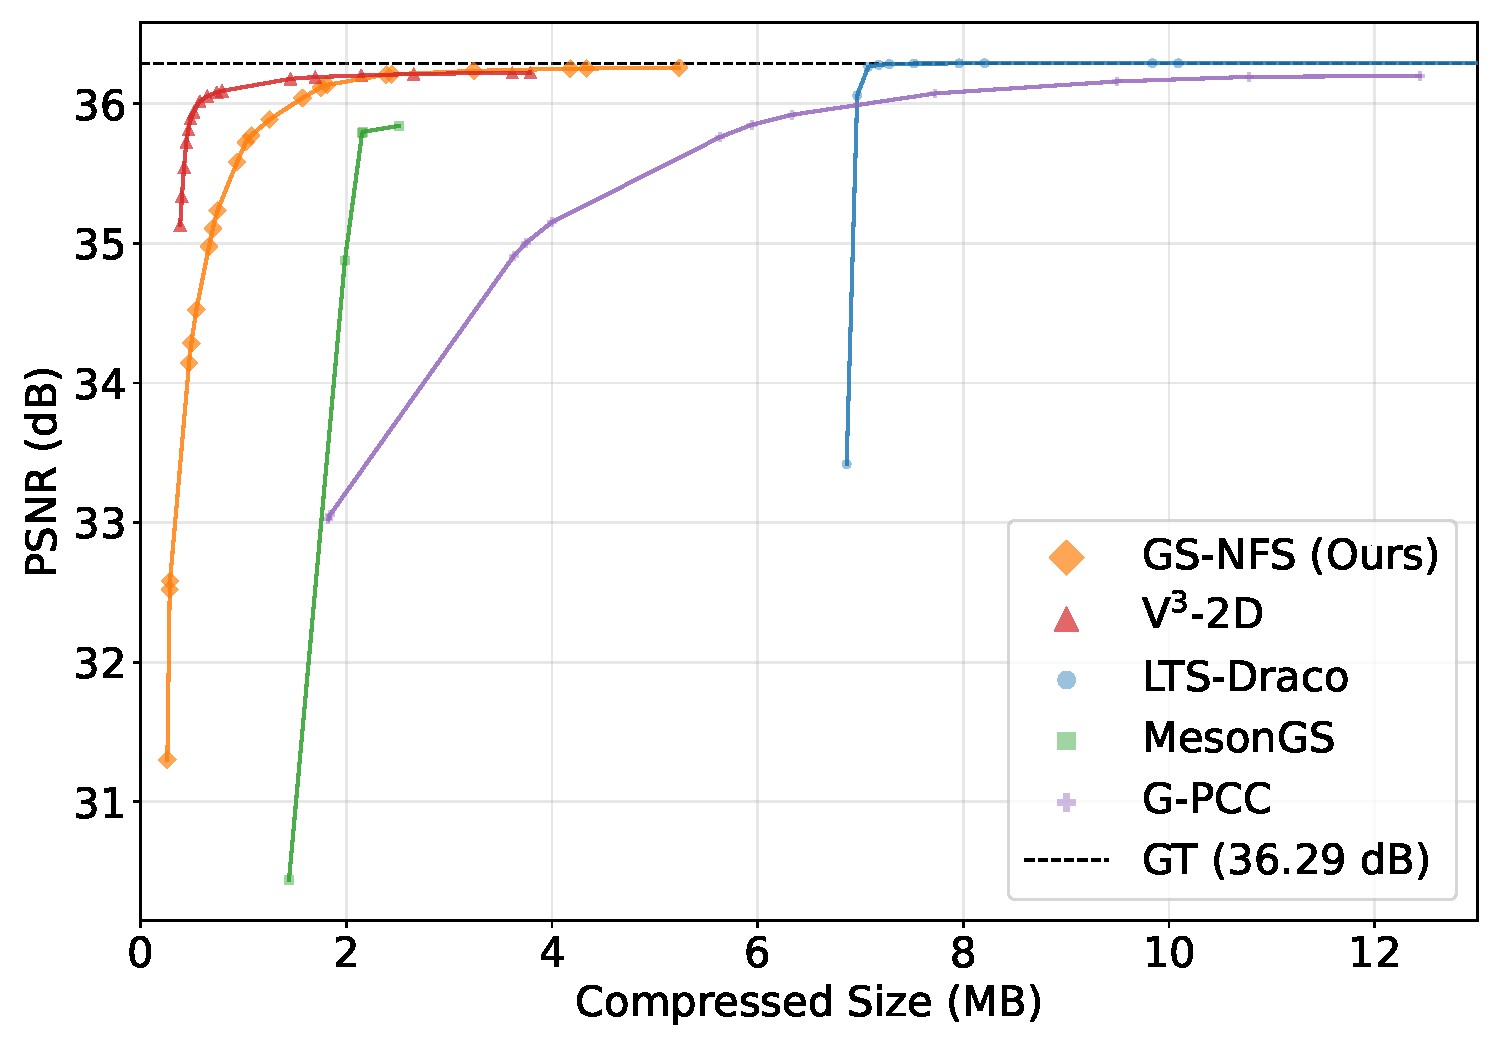
\includegraphics[width=\textwidth]{figures/rd_baselines/rd_baselines_curve_4K_Actor1_Greeting_frame0.pdf}
    \label{fig:rd-act1}
  \end{minipage}
  \begin{minipage}[t]{0.33\textwidth}
    \centering
    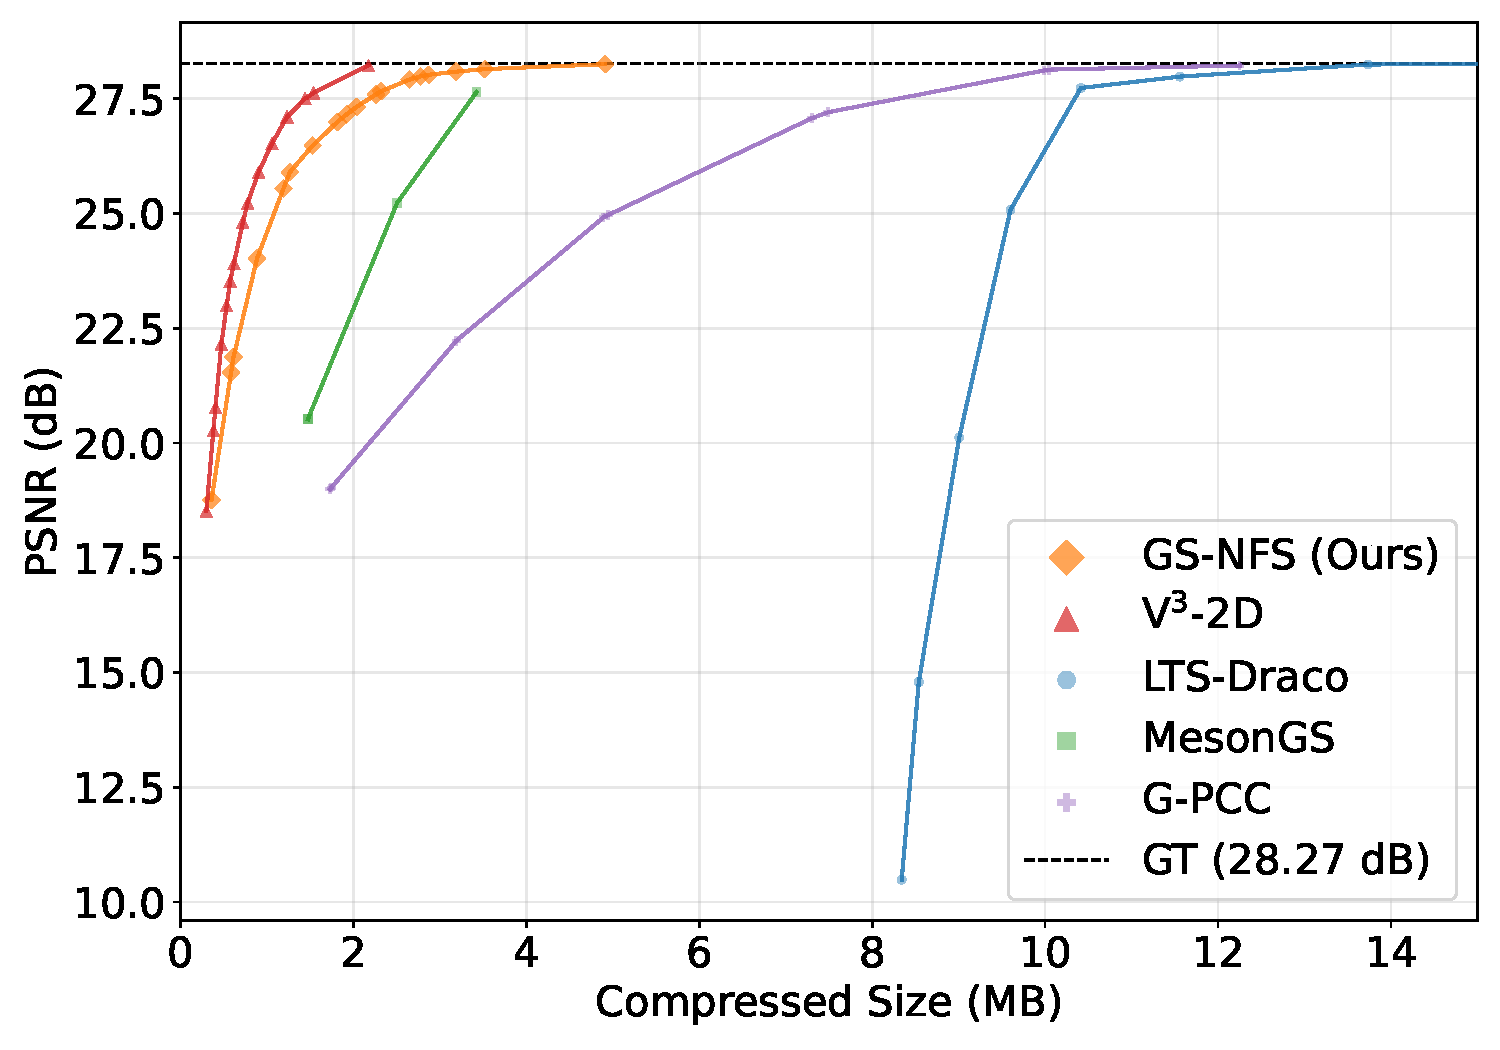
\includegraphics[width=\textwidth]{figures/rd_baselines/rd_baselines_curve_flame_salmon_1_frame1.pdf}
    \label{fig:rd-salmon}
  \end{minipage}
  \begin{minipage}[t]{0.33\textwidth}
    \centering
    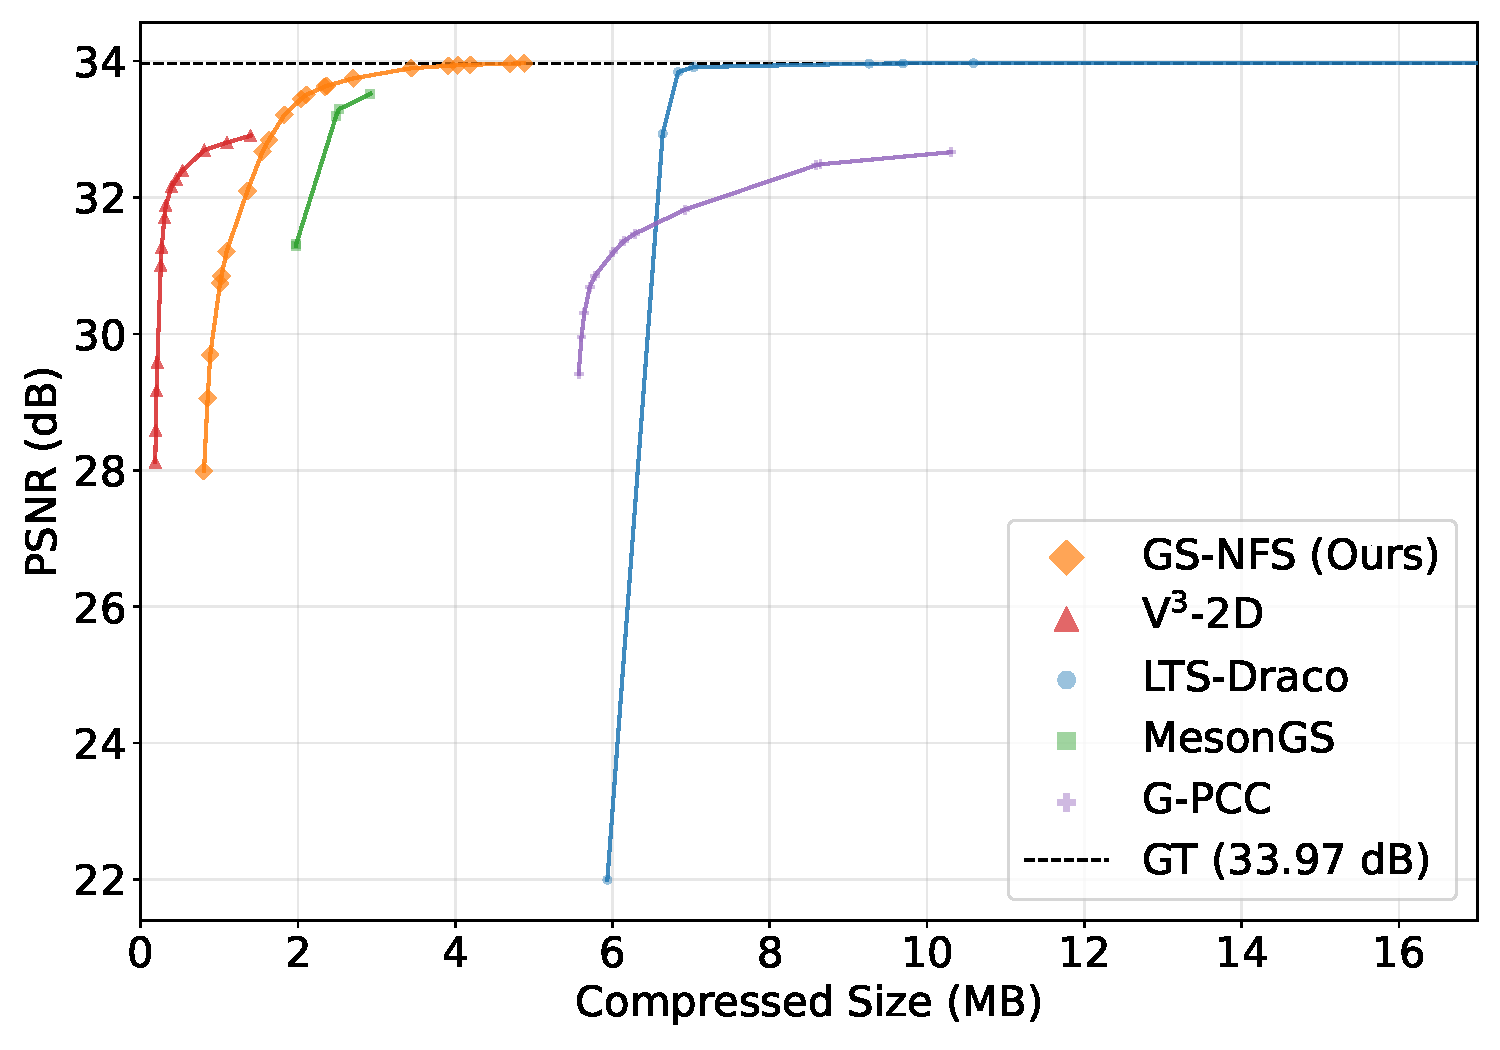
\includegraphics[width=\textwidth]{figures/rd_baselines/rd_baselines_curve_sear_steak_frame1.pdf}
    \label{fig:rd-steak}
  \end{minipage}
  \caption{R-D curves for (Left) Actor1 from HiFi4G, (Middle) flame\_salmon from N3DV, and (Right) sear\_steak from N3DV.}
  \vspace{-10pt}
  \label{fig:rd-curves}
\end{figure*}


To understand quality and compression trade-offs of different designs, we can also use a \textit{rate-distortion} curve or \textit{R-D curve}.
%
Such a curve plots \textit{rate} on the x-axis, \textit{quality} or distortion on the y-axis, and the curve represents the best quality one can obtain for a given rate.
%
To obtain this curve, practitioners explore a large space of codec parameters, obtain the rate and quality for each parameter, and plot these as points on the R-D plot.
%
The R-D curve is the \textit{convex hull} of those points.

R-D curves can also help encode videos at a given bitrate $B$.
%
To do this, we find the point on the convex hull whose rate is closest to $B$, and use its configuration to encode at the target bitrate.
%
We also used R-D curves to find the \gsnfs{} configuration with the nearest PSNR in \cref{sec:qual-compr-perf}.

\parab{Methodology.}
%
We computed R-D curves for the first frame of \textit{all} sequences, for all our baselines.
%
To do this, we sweep the space of parameters of each baseline and \gsnfs{}, plot rate and distortion and compute the convex hull as discussed above.
%
\cref{app:generating-r-d} discusses the parameters we used for each baseline and for \gsnfs{}.
%
For some approaches like MesonGS and G-PCC, we could not explore all parameter combinations because of their high encoding latency, and exploring the entire space would have taken hours or days.
%
In contrast, for \gsnfs{}, we were able to evaluate 1000 combinations in about 12 minutes.

%% %
%% \gsnfs's codec has the following parameter knobs: octree depth $J$ for position, quantization step size for attributes--rotation $\Delta_\mathrm{rot}$, scale $\Delta_\mathrm{sc}$, opacity $\Delta_\mathrm{opa}$, DC $\Delta_\mathrm{DC}$, and AC $\Delta_\mathrm{AC}$; position isn't quantized.
%% %
%% For each parameter combination, we encode, decode, render test views, and record PSNR, SSIM, and compressed size.
%% %
%% The convex hull of the resulting (size, PSNR) points forms the R--D curve and points on the hull define a bitrate ladder.

%% Because \gsnfs{} encodes and decodes each frame in ${\sim}20$~ms, sweeping large combination of the parameter space takes only minutes per frame on a single GPU.
%% %
%% By contrast, MesonGS would require \textit{days} to explore the same number of operating points.

\parab{R--D curves.}
%
\cref{fig:rd-curves} shows the R--D curves for one HiFi4G sequence (\textit{Actor1}) and two N3DV sequences (\textit{flame\_salmon\_1} and \textit{sear\_steak}).
%
\cref{fig:rd-baselines-hifi4g} and \cref{fig:rd-baselines-n3dv} depict the R-D curves for the remaining sequences for the two datasets respectively.
%
If the R-D curve for approach $A$ is entirely to the left of the curve for $B$, for a given sequence, we say that $A$ dominates $B$.
%
If the two curves intersect, then one is better in some bitrate regimes, and worse in others.

Consider the R-D curves for \textit{Actor1}.
%
Clearly, \gsnfs{} dominates MesonGS, Draco-LTS, and G-PCC.
%
However, \vthree{}-2D dominates \gsnfs{}: it can, for a given quality, encode at a lower rate than \gsnfs{}.
%
This explains why its compression performance was better in our baseline comparisons (\cref{sec:qual-compr-perf}), and is likely due to its use of 2D codecs' ability to do inter-frame compression.

The same is true for \textit{frame\_salmon}, except for this full-scene sequence, \vthree{}-2D's R-D curve is closer to, but still dominates \gsnfs{}'s.
%
For this sequence, both these approaches dominate MesonGS, Draco-LTS, and G-PCC.

On the other hand, for \textit{sear\_steak}, \vthree{}-2D does \textit{not} dominate \gsnfs{}.
%
In fact, for this sequence, and for \textit{three other sequences} in N3DV out of a total of six (cook\_spinach, cut\_roasted\_beef, and flame\_steak, \cref{fig:rd-baselines-n3dv}), \vthree{}-2D's R-D curve shows that \textit{there is no parameter setting for which its quality reaches close to the ground-truth PSNR} (we explored QP values from 1 to 40, where 1 is the best quality).

In each case, \gsnfs{} has a parameter setting that can provide \textbf{0.5--2 dB} higher PSNR for the same rate.
%
Moreover, for all of these sequences, \gsnfs{} has parameter settings that can reach ground-truth (GT) quality.
%
Put another way, if \gsnfs{} were used to encode videos for DASH-based \dgs{} streaming, for these sequences, it would provide much better quality at higher bandwidth-availability.

To our knowledge, \vthree{}-2D has only been evaluated on person-centric datasets and not on full-scene ones.
%
Now, \vthree{}-2D must map 3D Gaussian positions to a 2D image.
%
%If the 2D image resolution is small, or if the \gs{} frame has many Gaussians, then multiple Gaussians might map to the same frame.
%
%is \vthree{}-2D must pick one of these points, and if it picks this point incorrectly, visual quality can suffer.
%
%The N3DV sequences have many more Gaussians because they capture a full scene.
%
% New text AO
There are many possible 3D-to-2D mappings; \vthree{}-2D applies a fixed criterion to determine where an attribute corresponding to a Gaussian in 3D should be located in the 2D.
%
Consider two consecutive frames in 3D; the 3D-to-2D mapping algorithm is applied independently to each frame, which means that even if motion in the 3D scene is smooth, Gaussian attributes close to each other on the first 2D frame may not be close to each other in the second 2D frame. 
%
As a sequence, because the location of the same 3D attributes may change from one 2D frame to another, motion-compensated prediction in the 2D frames may not work well, potentially resulting in a higher rate than an intra-only approach. 
%
We conjecture that, for this reason, \vthree{}-2D does not perform well in some N3DV sequences, where inter-frame coding becomes inefficient.
%
On the other hand, \gsnfs{} does not exhibit this degradation because it uses a 3D codec.
%
% \ramesh{Antonio, please wordsmith as necessary.} 
% \ao{I edited the text above and commented the old version. I explained why I think there is some inefficiency; feel free to shorten. }
% \ao{We have observed a similar phenomenon in point clouds (VPCC). Eduardo/Haoran: Is there some reference in the VPCC literature for this? }

%% \parab{Bitrate ladder.}
%% From the R--D curves, we extract \note{XX} operating points on the convex hull spanning the useful rate range.
%% %
%% \cref{tab:bitrate-ladder} shows a representative ladder for \note{XX} sequences.
%% %
%% The lowest-rate point achieves \note{$>$XX$\times$} compression with modest quality loss (${\sim}2$~dB PSNR drop), while the highest-rate point preserves quality within 0.1~dB of the uncompressed model.
%% %
%% This range of operating points enables adaptive streaming: the server can select the appropriate representation based on the client's available bandwidth, analogous to DASH-based 2-D video delivery.

%% \begin{table}[t]
%%   \centering
%%   \footnotesize
%%   \begin{tabular}{cccccccc}
%%     \hline
%%     \textbf{Depth $J$} & \textbf{$\Delta_\mathrm{sc}$} & \textbf{$\Delta_\mathrm{rot}$} & \textbf{$\Delta_\mathrm{opa}$} & \textbf{$\Delta_\mathrm{DC}$} & \textbf{$\Delta_\mathrm{AC}$} & \textbf{Size (MB)} & \textbf{PSNR (dB)} \\
%%     \hline\hline
%%     \note{X} & \note{X} & \note{X} & \note{X} & \note{X} & \note{X} & \note{X} & \note{X} \\
%%     \hline
%%   \end{tabular}
%%   \caption{Representative bitrate ladder. \raj{sample from csv. Move to appendix to save space}}
%%   \label{tab:bitrate-ladder}
%% \end{table}

\subsection{Mobile Performance}\label{sec:mobile-performance}
% Pick datasets:
%% \begin{outline}
%%   \begin{itemize}
%%   \item Decode performance for different datasets/videos on Jetson
%%   \item Rendering speed on iOS device
%%   \end{itemize}
%% \end{outline}

\gsnfs{} supports \dgs{} playback on resource-constrained devices.
%
To demonstrate this, we evaluate \gsnfs{}'s decode performance on an NVIDIA Jetson Orin, a mobile GPU with compute comparable to those in in AR/VR headsets and edge devices~\cite{nvidia_jetson_orin}.
%
%\eduardo{missing reference above}
\cref{tab:jetson-decode} shows end-to-end decode latency on Jetson Orin.
%
We observed that many \gs{} mobile implementations can support 30 fps \gs{} rendering for Gaussians with only SH DC coefficients (SH0), but not at higher SH degrees~\cite{v3volumetric}.
%
At SH0, \gsnfs{} achieves 40--59~ms across all sequences, allowing about $17$--$25$~fps decoding.
%
Latency scales \emph{sub-linearly} with channel count: going from SH0 to SH3 (5.1$\times$ more channels) increases average decode latency across all sequences by ${\sim2}\times$.
%
At higher SH degrees, scene complexity dominates for full-scene content (more Gaussians): flame\_salmon at SH2 (35~ch) is $2\times$ slower than Actor1 at SH3 (56~ch), despite having fewer channels.

\begin{table}[t]
  \centering
  % \footnotesize
  \begin{tabular}{l|l|r|r}
    \hline
    \textbf{Sequence} & \textbf{SH degree} & \textbf{\# channels} & \textbf{Decode latency (ms)}\\
    \hline\hline
    Actor1         & 0 & 11 & 40 \\
    Actor1         & 3 & 56 & 57 \\
    flame\_salmon  & 0 & 11 & 59 \\
    flame\_salmon  & 2 & 35 & 120 \\
    sear\_steak    & 0 & 11 & 49 \\
    sear\_steak    & 2 & 35 & 113 \\
    \hline
  \end{tabular}
  \caption{Decode latency on Jetson Orin, averaged across frames.}
  \label{tab:jetson-decode}
\end{table}

\subsection{Novel \gsnfs{} Use Cases}\label{sec:other-capabilities}

%% \begin{outline}
%%   \begin{itemize}
%%   \item Large static scene compression: compare against MesonGS, LTS, G-PCC, 2d-png [R]
%%   \item GPS-Gaussian: run at x fps, and show that we can compress in real-time [*]
%%   \item (Stretch) Point cloud compression [*]
%%   \end{itemize}
%% \end{outline}

So far, we have discussed using \gsnfs{} to compress stored \dgs{} videos.
%
In this section, we demonstrate that \gsnfs{} can \textbf{compress, on-the-fly, live \dgs{} videos} generated by feed-forward Gaussian generators and \textbf{point-clouds} as well, both at full frame-rate.
%
% This is an important reason why fast encoding matters (\cref{sec:appr-chall-contr}).
% %
% We also demonstrate that \gsnfs{} can compress \textbf{point clouds} at over 30~fps.
% % \ao{compress at frame-rate is unclear. Compress at high frame rates? Compress at the input frame rate? Compress in real time? Also, the sentence above discusses point clouds, but the sentence below mentions post-training, which is not applicable to point clouds; it applies only to 3DGS.}
% %
% To our knowledge, no other point-cloud compression technique can match this performance.
%
\cref{app:compr-stat-scen} also demonstrates \gsnfs{}'s ability  to quickly compress large static \gs{} scenes.

\parab{Live \dgs{} Compression.}
%
GPS-Gaussian~\cite{zheng2024gpsgaussian} generates Gaussian at ${\sim}25$~fps (${\sim}270$K Gaussians per frame) using captures from 2 views of a person.
%
We adapted \gsnfs{} to compress these frames on-the-fly.
%
Specifically, our approach repeatedly takes 2 views of a person per frame (pre-loaded from disk), generates a \gs{} frame using GPS-Gaussian, compresses the frame using \gsnfs{}, and finally decompresses the frame to reconstruct the \gs frame.
%
This pipeline can achieve \textbf{22~fps} and an end-to-end latency (from capture to after decode) of \textbf{75~ms}.
%
While \gsnfs's encoder and decoder takes only $15$~ms each, the GPS-Gaussian generator takes ${\sim}43$~ms, and is the bottleneck in this pipeline.

\parab{Point cloud compression.}
%
Since \gsnfs{} builds upon G-PCC, it can compress point clouds (\gs with only DC attribute).
%
So, we evaluate its performance on popular point cloud-based volumetric video datasets.
%
We use six sequences from two datasets: four single person sequences from 8i~\cite{8i-ptcl} (${\sim}700$K--1M points/frame; ${\sim}17$--$26$~MB) and 2 multi-person full-scene sequences from CMU Panoptic~\cite{cmu-panoptic} (${\sim}700$K--850K points/frame; ${\sim}17$--$21$~MB).
%
Point clouds are voxelized at octree depth $J\!=\!10$ and \gsnfs{}'s codec uses a quantization step $0.1$ for color attributes.
% \ao{best quality with least size is confusing: you cannot optimize both simultaneously.}
%
\gsnfs{} can encode each frame in $12$--$14$~ms and decode in $9$--$12$~ms while achieving \textbf{lossless geometry} and color Y-PSNR of $31$--$37$~dB. 
%
It can compress 8i sequences to $270$--$370$~KB and CMU Panoptic sequences to $660$--$780$~KB, \textbf{26--64$\times$} smaller than the original size.
%\raj{Ramesh: Do we need to compare against Draco and G-PCC?}

\subsection{Ablations}\label{sec:ablations}

% We demonstrate the importance of color de-correlation (\cref{sec:klt}) and that of CUDA optimizations for RAHT on Jetson (\cref{sec:gpu-raht}).
%

\parab{KLT color decorrelation.}
%
\gsnfs{} decorrelates SH coefficients using a YUV transform followed by a per-channel KLT (\cref{sec:klt}).
%
%\ao{Broken reference above}
%
\cref{tab:ablation-klt} shows the impact on compressed size.
%
RGB inflates the attribute bitstream by \textbf{43\%} compared to raw RGB, while YUV is larger than KLT by \textbf{36\%} for flame\_salmon.
%
For others, the reductions are smaller, but still significant.
%
The additional latency for computing and applying the KLT matrix is less than 1~ms per frame, a negligible overhead.
%
%% Beyond compression, KLT decorrelation concentrates energy in the first few AC coefficients, 

\parab{CUDA vs.\ PyTorch RAHT decode on Jetson.}
%
RAHT takes about ${\sim}50$\% of the per frame decode latency, particularly on Jetson Orin.
%
An efficient implementation of RAHT is crucial for mobile decode.
%
\gsnfs{}'s custom CUDA RAHT kernels achieve $2.0$--$3.9\times$ speedup over a PyTorch baseline on Jetson, with larger gains for lower SH degrees (\cref{tab:jetson-raht-decode}).
%
We see a reduction of about $4$--$5\times$ for SH0 and $2$--$4\times$ for higher SH degrees for RAHT decode, which is the main bottleneck for mobile decode; prelude has ${\sim}2\times$ of speedup, since it doesn't depend on the number of channels.
%
These gains also reduce encode latency, since both forward and inverse RAHT perform the same work.

\parab{Other Ablations.}
\cref{app:other-ablations} describes the cost of CPU octree coding (\cref{sec:gpu-octree}), and explores RLGR parameter sensitivity of (\cref{sec:quant-entr-coding}).

%% \begin{comment}
%% LiVoGS J=15  qs=0.0001  color_space=rgb  nvcomp=ANS
%% Pipeline throughput: 22.0 FPS (45.49 ms/frame)
%%   Per-stage summary (skipping first 5):
%%   Stage             Mean ms    Std ms       FPS
%%   ---------------------------------------------
%%   generation          42.88      0.22      23.3
%%   upload               2.08      0.21     481.9
%%   encode              14.79      0.38      67.6
%%   decode              14.82      0.70      67.5
%%   e2e (sum)           74.56      1.08      13.4
%%   e2e (wall)          84.01      1.51      11.9
%% \end{comment}

%% \parab{iOS rendering.}
%% \note{TODO: Measure rendering speed on iOS device.}

%% ====================================================================
%
%% \begin{outline}
%%   Compression:
%%   \begin{itemize}
%%   \item CPU vs GPU implementation of Octree [R]
%%   \item Impact of octree [H] 
%%   \item Coarse parallelization of RLGR and CPU version of RLGR [R]
%%   \item Importance of CUDA optimizations (CUDA vs Pytorch): For RAHT, important for decode [H]
%%   \end{itemize}

%%   Bandwidth Adaptivity/Decorrelation [H]
%%   \begin{itemize}
%%   \item With and without RGB->YUV
%%   \item With and without KLT decorrelation
%%   \end{itemize}
%% \end{outline}
%



%% ====================================================================
